\documentclass%
%[handout]
{beamer}
% % % % % % % %
% % % % % % % %
% % % % % % % %
%IMPORTANT
%compiles with
%pdflatex -shell-escape
%IMPORTANT
% % % % % % % %
% % % % % % % %
% % % % % % % %
\mode<presentation>
{
\useinnertheme{rounded}
\useoutertheme{infolines}
\usecolortheme{orchid}
\usecolortheme{whale}
}

\usepackage[english]{babel}
\usepackage[latin1]{inputenc}
\usepackage[all,cmtip]{xy}
\usepackage{times}
\usepackage[T1]{fontenc}
\usepackage{../example-templates}
\usepackage{../pstricks-commands}

\usepackage{auto-pst-pdf}
\usepackage{pst-plot}
%\usepackage{pstricks-add}

% Or whatever. Note that the encoding and the font should match. If T1
% does not look nice, try deleting the line with the fontenc.


\graphicspath{{../../modules/}}

\newtheoremstyle{partialproof}{3pt}{3pt}{}{}{}{.}{.5em}{}
\theoremstyle{partialproof} \newtheorem{partialproof}[theorem]{Proof.}
%\DeclareMathOperator{\diff}{d}
\setbeamertemplate{navigation symbols}{}

\includeonlylecture{1}

\newcommand{\lect}[3]{
  \date{#1}
  \lecture[#1]{#2}{#3}
}

\setbeamertemplate{footline}
{
  \leavevmode%
  \hbox{%
  \begin{beamercolorbox}[wd=.333333\paperwidth,ht=2.25ex,dp=1ex,center]{author in head/foot}%
    \usebeamerfont{author in head/foot}\insertshortauthor
  \end{beamercolorbox}%
  \begin{beamercolorbox}[wd=.333333\paperwidth,ht=2.25ex,dp=1ex,center]{title in head/foot}%
    \usebeamerfont{title in head/foot}\insertshorttitle
  \end{beamercolorbox}%
  \begin{beamercolorbox}[wd=.333333\paperwidth,ht=2.25ex,dp=1ex,center]{date in head/foot}%
    \usebeamerfont{date in head/foot}\insertshortdate{}
  \end{beamercolorbox}}%
  \vskip0pt%
}

% If you have a file called "university-logo-filename.xxx", where xxx
% is a graphic format that can be processed by latex or pdflatex,
% resp., then you can add a logo as follows:

%\pgfdeclareimage[height=0.8cm]{logo}{bluelogo}
%\logo{\pgfuseimage{logo}}
\renewcommand{\Arcsin}{\arcsin}
\renewcommand{\Arccos}{\arccos}
\renewcommand{\Arctan}{\arctan}
\renewcommand{\Arccot}{\text{arccot\hspace{0.03cm}}}
\renewcommand{\Arcsec}{\text{arcsec\hspace{0.03cm}}}
\renewcommand{\Arccsc}{\text{arccsc\hspace{0.03cm}}}



\begin{document}

\AtBeginLecture{%

\title[\insertlecture]{FreeCalc}
\subtitle{\insertlecture}
\author[FreeCalc]{}
\institute[UMass Boston]{University of Massachusetts Boston}
\date{\insertshortlecture}
\begin{frame}
  \titlepage
\end{frame}
}%

% begin lecture
\lect{\today}{Sample}{1}{
\begin{frame}
\begin{example}
\begin{columns}
\column{0.35\textwidth}
\uncover<2->{
\begin{pspicture}(-1.7,-0.7)(1.7,3)
\fcBoundingBox{-1.7}{-0.7}{1.7}{3}
\fcAxesIIId{2}{2}{2}
\fcCurveIIId[plotpoints=500, linecolor=red]{0}{1080}{[t cos t sin t 360 div]}
\end{pspicture}
}
\column{0.65\textwidth}
Let $\fcv{r}(t) = ( \cos{t}, \sin{t}, t)$  \uncover<2->{(the curve is called a \alert<2>{helix} - (not a spiral) ).}
\begin{itemize}
\item \alert<1>{Do you know the name of this curve?}
\item Find the arclength function.
\item Find the length of the segment of the curve given by $t\in [0,2\pi]$.
\end{itemize}
\end{columns}


\[
\begin{array}{rcl}
\uncover<3->{\fcv{r}'(t) &=& ( -\sin{t}, \cos{t}, 1 ) \\}
\uncover<4->{\fcv{r}'(t)| &= &\sqrt{2}\quad .}
\end{array}
\]
\uncover<5->{
Therefore the arclength function is
\[
\begin{array}{rcl}
L(t) &=&\displaystyle \int_0^t |\fcv{r}'(\tau)| \diff \tau \\
\uncover<6->{& =& t\sqrt{2} \quad  .}
\end{array}
\]
}
\end{example}
\end{frame}


%\begin{frame}
Notation: $\fcv T$- unit tangent vector, $\fcv r$- position vector.
\begin{example}
Compute the curvature of $\fcv{r}(t) = \langle \cos{t}, \sin{t}, t\rangle$
$\fcv{r}'(t) = \langle -\sin{t}, \cos{t}, 1 \rangle \Longrightarrow|\fcv{r}'(t)| = \sqrt{2}$;

$\fcv{T}(t) = \frac{1}{\sqrt{2}}
\langle -\sin{t}, \cos{t}, 1 \rangle
\Longrightarrow
\fcv{T}'(t) = \frac{1}{\sqrt{2}}
\langle -\cos{t}, -\sin{t}, 0 \rangle
\Longrightarrow $
$|\fcv{T}'|=\frac{1}{\sqrt{2}}$

Curvature:
%
$$\kappa(t) = \frac{|\fcv{T}'(t)|}{|\fcv{r}'(t)|} =
\frac{1}{2}\; .$$ 


Alternatively: $\fcv{r}''= \langle -\cos{t}, -\sin{t}, 0 \rangle$,
%
$$\fcv{r}'' \times \fcv{r}' = \left|
\begin{array}{ccc}
\fcv{i} & \fcv{j} & \fcv{k} \\
-\cos{t}&  -\sin{t}&  0 \\
-\sin{t}& \cos{t}& 1
\end{array}
\right| = -\sin{t} \, \fcv{i} +
\cos{t}\, \fcv{j} -\fcv{k} $$
%
$$\kappa(t) =
\frac{|\fcv{r}''(t) \times \fcv{r}'(t)|}
{|\fcv{r}'(t)|^3} =
\frac{\sqrt{2}}{(\sqrt{2})^3} = \frac{1}{2}\; .$$
\end{example}
\end{frame}
%\begin{frame}
\begin{example}
Let $\fcv r(t)$ be the coordinate curves for the spherical coordinates, i.e., let
\[
\begin{array}{rcl}
\fcv{e}_\rho(t)&=& \alertNoH{2,3}{ ( t\sin \phi \cos \theta, t\sin \phi \sin \theta, t\cos \phi ) }\\
\fcv{e}_\phi(t)&=& \alertNoH{4,5}{ ( \rho\sin t \cos \theta, \rho\sin t \sin \theta, \rho\cos t ) }\\
\fcv{e}_\theta(t)& =& \alertNoH{6,7}{( \rho\sin\phi \cos{t}, \rho\sin\phi \sin{t}, \rho\cos\phi) }\\
\end{array}
\]
where $\rho$, $\phi$, $\theta$ are regarded as constants and $t$ as the curve parameter. Find $\fcv {e}_\rho'(t)$, $\fcv e_\phi'(t)$, $\fcv e_\theta'(t)$. Compute $ (\fcv e_\rho '(\rho) \times \fcv e_{\theta}'(\theta) )\cdot \fcv e_{\phi}'(\phi)$.

\[
\begin{array}{rcl}
\uncover<2->{\alertNoH{2,3,8}{ \fcv{e}_\rho '(t)} &\alertNoH{2,3}{=}&\uncover<3->{\alertNoH{3,8}{ ( \sin \phi \cos \theta, \sin \phi\sin \theta, \cos \phi ) }}\\}
\uncover<4->{\alertNoH{4,5,9}{\fcv e_{\phi}'(t)} &\alertNoH{4,5}{=}&\uncover<5->{ \alertNoH{5,9}{ ( \rho\cos t \cos\theta, \rho\cos t \sin\theta, -\rho\sin t )}} }\\
\uncover<6->{\alertNoH{6,7,10}{\fcv e_{\theta}'(t)} &\alertNoH{6,7}{=}&\uncover<7->{ \alertNoH{7,10}{ ( -\rho\sin \phi \sin t, \rho\sin \phi \cos t, 0 )}} }\\
\uncover<8->{
(\fcv{e}_{\rho}'(\rho) \times \fcv{e}_{\phi}'(\phi)) \cdot \fcv{e}_{\theta}'(\theta) &=&\alertNoH{11,12}{ \left| \begin{array}{ccc}
\alertNoH{8}{ \sin \phi \cos \theta }& \alertNoH{8}{\sin \phi \sin\theta }&  \alertNoH{8}{\cos\phi} \\
\alertNoH{9}{\rho \cos \phi \cos \theta }&\alertNoH{9}{ \rho \cos \phi\sin \theta }&\alertNoH{9}{ -\rho \sin \phi} \\
\alertNoH{10}{-\rho \sin \phi\sin \theta }&\alertNoH{10}{ \rho \sin \phi \cos \theta }&\alertNoH{10}{0}
\end{array}\right|} \\}
\uncover<11->{&\alertNoH{11,12}{=}&\uncover<12->{\alertNoH{12}{\rho^2\sin\phi }}}
\end{array}
\]
\end{example}
\end{frame}

%\begin{frame}
\begin{itemize}
\item An analytical description is technically best, but not easy to interpret.
\item If output is a scalar, where does the function attain its extreme values (maxima, minima)?  
\item How do values change for nearby points - are they decreasing, increasing, how fast?
\item We will learn to decode this information from the analytical descriptions.
\item Even so, ``a picture is worth a thousand words (and, say, 10 f-las)''.
\end{itemize}
\end{frame}

\begin{frame}
\begin{center}
\psset{xunit=1cm,yunit=1cm}
\begin{pspicture}(-3,-3)(3,5.5)
\renewcommand{\fcScreen}{[-1 -1 -0.4] 0}
\fcAxesIIId{5}{5}{5}
\fcPlotIIId[linewidth=0.3pt, linecolor=blue]{iterationsX=50, iterationsY=50}{-4}{-4}{4}{4}{ x 3 exp x y 4 exp mul add x 5 div sub 10 mul 2.729 x dup mul y dup mul add neg exp mul 2.729 x 1.225 sub dup mul y dup mul add neg exp add}
\rput[t](-3,5.3){Graph of a scalar function.}
\end{pspicture}
\end{center}

\end{frame}

\begin{frame}\frametitle{Graph of a function}
\begin{itemize}
\item For one variable function, $y=f(x)$, the graph of $f$ is a set of points in $\RR^2$: the set of points $(x,y)$ such that $y=f(x)$.
\item Example: if $f(x) = x^2$, then  $(3,9)$ is on the graph, because $9=3^2$, but $(2,5)$ is not because $5 \neq 2^2$.
\item We can extend this graphical representation for functions with two dimensional input and one dimensional (scalar) output. 
\item The \emph{graph} of the function $f\colon D \to \RR$, where $D$ is a region in $\RR^2$, is the set of points $P(x,y,z)$ in $\RR^3$ whose coordinates satisfy the condition 
\[
z=f(x,y)\quad .
\]
\item For example, the graph of $f(x,y) = 2x-y+3$ is the set
\[
\{ (x,y,z) \, | \, z= 2x-y+3\} \Longrightarrow \text{ plane } 2x-y-z+3=0 \; .
\]

\end{itemize}

 



\end{frame}


%\begin{frame}
\begin{pspicture}(-1, -1)(2,2)
\fcBoundingBox{-1}{-1}{2}{2}
\fcSurfaceDirectDraw{iterationsX=10, iterationsY=10, Delta=1}{-90}{-1}{90}{1}{[u cos u sin v]}
\end{pspicture}
\begin{pspicture}(-1, -1)(2,2)
\fcBoundingBox{-1}{-1}{2}{2}
\fcStartIIIdScene %
\fcSurfaceInScene[iterationsU=7, iterationsV=4]{0}{-1}{300}{1}{[u cos u sin v]}
\fcFinishIIIdScene
\end{pspicture}
\end{frame}

%\begin{frame}
We have the ellipsoid 
\[
\frac{x^2}{a^2}+\frac{y^2}{b^2}+\frac{z^2}{c^2}= 1.
\]
We are seeking to project it orthographically onto the plane 
\[
px+qy+rz=s.
\]
The direction in which our ``orthographic eye'' is looking is $\fcv n= (p,q,r)$.
\end{frame}
\begin{frame}
\begin{pspicture}(0,0)(0,0)%
%\renewcommand{\fcScreenStyle}{x}%
%\renewcommand{\fcScreen}{[-1 1 2] 0}
\fcAxesIIId{5}{5}{5}%
\fcStartIIIdScene%
%\fcCurveIIIdBlockedByScreen{0}{360}{[t cos t sin 0]}{\fcScreenWithSpace pop 0}
\fcEllipsoid[linecolor=red]{0 0 0 3 2 1}%
%\fcCone{-2 2 0 0 0 1 1 1}
\renewcommand{\fcIterationsX}{15}
\renewcommand{\fcIterationsY}{15}
\fcFinishIIIdScene%
\end{pspicture}
\end{frame}

%\begin{frame}
\frametitle{Continuity}
\begin{definition}
Suppose
\begin{itemize}
\item $\fcv{r}$ is defined at $t_0$
\item<2-> $\lim\limits_{t\to t_0} \fcv{r}(t)$ exists.
\end{itemize}
\uncover<3->{
Then we say that $\fcv{r} \colon [a,b] \to \RR^3$ is continuous at $t_0$ if
\[
\lim_{t\to t_0} \fcv{r}(t) = \fcv{r}(t_0)\quad .
\]
}
\end{definition}
\begin{observation}
$\fcv{r}(t) = \langle x(t), y(t), z(t) \rangle$ is continuous at $t_0$ $\Longleftrightarrow$ $x(t), y(t), z(t) $ are all continuous at $t_0$.

\end{observation}  
  

\end{frame}
%
\begin{frame}
\frametitle{Limits}
\begin{definition}
We say that $$\lim_{t\to a} \fcv{r}(t) = \fcv{u}$$ if \alertNoH{4}{ by selecting that } $t\neq a$ be close enough to $a$ \alertNoH{5}{we can guarantee that $\fcv{r}(t)$} \alertNoH{3}{is as close to $\fcv{u}$ as we want}.

\medskip

\uncover<2->{In strict mathematical language: $\lim_{t\to a} \fcv{r}(t) = \fcv{u}$ if \alertNoH{3}{for every $\varepsilon >0$} \alertNoH{4}{there exists $\delta>0$} \alertNoH{5}{ such that for all $t$ with $0<|t-a|<\delta $} \alertNoH{3}{we have that $| \fcv r(t)-u|<\varepsilon $}.}
\end{definition}
\end{frame}

\begin{frame}
\begin{itemize}
\item We define the ``postman distance'' between $(x_1,y_1,z_1)$ and $(x_2, y_2, z_2)$ to be the number $\max(|x_1-x_2|, |y_1-y_2|, |z_1-z_2|) $.
\item<2-> Two points in Euclidean distance are close if and only if they are close in ``postman distance''.
\item<3-> Unlike higher dimensions, in dimension 1 postman distance coincides with Euclidean distance.
\item<4-> Let $\fcv{r}(t) = ( x(t), y(t), z(t) )$ and $\fcv{u}=( u_1,u_2,u_3)$.
\item<5-> Then
\[
\lim_{t\to a} \fcv{r}(t) = \fcv{u} \Longleftrightarrow
\left|
\begin{array}{l}
\lim\limits_{t\to a} x(t) = u_1\\
\lim\limits_{t\to a} y(t) = u_2\\
\lim\limits_{t\to a} z(t) = u_3\\
\end{array}
\right.\quad .
\]
\end{itemize}
\end{frame}

%\makeatletter
\psset{xunit=1.1cm, yunit=1.1cm}
\begin{pspicture}(-2.2,-3.9)(2.345,3.234)
%\fcSet{shiftX=-3.1, shiftY=-2.8}
\fcBoundingBox{-2}{-2}{2}{2}
\fcLine{[0 0 ]}{[0 1]}
\fcLine{[0 0 ]}{[1 0]}
\psline(0, 0)(0,-1)
\psline(0.5, 0)(-1,0)

\end{pspicture}
\makeatother
\begin{frame}
\end{frame}
%\begin{frame}
\begin{pspicture}(-1, -1)(2,2)
\fcBoundingBox{-1}{-1}{2}{2}
\fcSurfaceDirectDraw{iterationsX=10, iterationsY=10, Delta=1}{-90}{-1}{90}{1}{[u cos u sin v]}
\end{pspicture}
\begin{pspicture}(-1, -1)(2,2)
\fcBoundingBox{-1}{-1}{2}{2}
\fcStartIIIdScene %
\fcSurfaceInScene[iterationsU=7, iterationsV=4]{0}{-1}{300}{1}{[u cos u sin v]}
\fcFinishIIIdScene
\end{pspicture}
\end{frame}

%\begin{frame}
\begin{pspicture}(-2,-2)(2,2)
%\pstVerb{[1 5 6]  \fcArrayToStack stack}
\pstVerb{[1 2 3] \fcProjectOntoScreen ==}
\pstVerb{[1 2 3] [4 5 6] \fcVectorMinusVector ==}
%\fcFullDot{1}{1}
%\pstVerb{[1 2 3] 5 \fcVectorTimesScalar \fcArrayToStack stack}
%\pscircle*[fillcolor=white, linecolor=red](! \fcProjectOriginOnPlane{1}{1}{1}{1}){0.07}
\end{pspicture}
\end{frame}
%

\begin{frame}
\frametitle{Constant Coordinate Sets}
\begin{columns}
\column{0.55\textwidth}
\psset{xunit=2.5cm, yunit=2.5cm}
\begin{pspicture}(-1, -1)(2,2)
\tiny%
\renewcommand{\fcScreen}{[-3 -1 -1] 0}%
\fcBoundingBox{-1.2}{-1.2}{2}{2}%
\fcLineIIId[arrows=->]{[0 0 0]}{[1.5 0 0]}%
\fcLineIIId[arrows=->]{[0 0 0]}{[0 1.5 0]}%
\fcLineIIId[arrows=->]{[0 0 0]}{[0 0 1.5]}%
\pstVerb{3 dict begin%
/xPoint 0.5 sqrt def%
/yPoint 0.5 sqrt def%
/zPoint 1 def%
}%
\multido{\na=1+1}{6}{\only<\na-7>{\pstVerb{%
/xPoint 1 \na\space 1 sub 10 div sub def%
/yPoint xPoint def%
}}%
\uncover<\na-6>{%
\fcDotIIId[linecolor=gray]{[1 \na\space 1 sub 10 div sub dup 1]}%
}%
}%
\multido{\na=8+1}{6}{\only<\na-14>{\pstVerb{%
\na\space 7 sub 12 mul dup
/xPoint exch cos def%
/yPoint exch sin def%
}}%
\uncover<\na-13>{%
\fcDotIIId[linecolor=gray]{[\na\space 7 sub 12 mul dup cos exch sin 1]}%
}%
}%
\multido{\na=15+1}{6}{\only<\na-21>{\pstVerb{%
/zPoint \na\space 15 sub -0.2 mul 1.2 add def%
}}%
\uncover<\na-20>{%
\fcDotIIId[linecolor=gray]{[xPoint yPoint \na\space 15 sub -0.2 mul 1.2 add]}%
}%
}%
\fcPerpendicularIIId[linestyle=dashed]{[xPoint yPoint zPoint]}{[0 0 1]}{0.2}%
\fcLineIIId{[0 0 0]}{[xPoint yPoint zPoint]}%
\fcPerpendicularIIId{[xPoint yPoint zPoint]}{[xPoint yPoint 0]}{0.2}%
\fcPutIIId[bl]{[xPoint yPoint zPoint]}{$~~P(x, y, z)$}
\fcPutIIId[tl]{[xPoint yPoint 0]}{$~~Q$}
\fcPerpendicularIIId[linestyle=dashed]{[xPoint yPoint 0]}{[1 0 0]}{0.2}%
\fcPerpendicularIIId[linestyle=dashed]{[xPoint yPoint 0]}{[0 1 0]}{0.2}%
\fcLineIIId{[0 0 0]}{[xPoint yPoint 0]}%
\fcPutIIId[r]{[xPoint 2 div 0 0]}{$x~~$}
\fcPutIIId[b]{[0 yPoint 2 div 0]}{$y$}
\fcPutIIId[r]{[0 0 zPoint 2 div]}{$z~~$}
\fcDotIIId{[xPoint yPoint zPoint]}%
\fcDotIIId{[xPoint yPoint 0]}%
\fcPutIIId[tr]{[xPoint 2 div yPoint 2 div 0]}{$r$}%
\fcAngleIIId[arrows=->, linecolor=red]{[1 0 0]}{[xPoint yPoint 0]}{0.3}%
\fcPutIIId[t]{[xPoint xPoint mul yPoint yPoint mul add sqrt dup xPoint exch div 0.4 mul exch yPoint exch div 2 div 0.4 mul 0]}{$\theta$}%
\uncover<7>{%
\fcLineIIId[arrows=->, linecolor=red]{[0 0 1]}{[1.4 1.4 1]}%
}%
\uncover<14>{%
\fcCurveIIId{-180}{180}{t cos t sin 1}%
}%
\uncover<21>{%
\fcLineIIId[linecolor=red]{[0.5 sqrt dup -0.2]}{[0.5 sqrt dup 1.5]}%
}%
\uncover<23>{%
\fcSurfaceIIId[linecolor=red]{iterationsX=11, iterationsY=11}{0}{-0.4}{180}{1}{u cos u sin  v}%
}%
\uncover<25>{%
\fcSurfaceIIId[linecolor=red]{iterationsX=11, iterationsY=17}{0}{-0.4}{1.6}{1.2}{u u v}%
}%
\uncover<27>{%
\fcSurfaceIIId[linecolor=red]{iterationsX=11, iterationsY=13}{0}{-180}{1.2}{180}{v sin u mul v cos u mul 1}%
}%
\pstVerb{end}%
\end{pspicture}
\column{0.45\textwidth}
What curve is traced when:
\begin{itemize}
\item \alert<1-7>{keep $\theta, z$ constant, let $r $ vary:} \uncover<7->{\alert<7>{horizontal ray;}}
\item \alert<8-14>{keep $r, z$ constant, let $\theta$ vary:} \uncover<14->{\alert<14>{horizontal circle;}}
\item \alert<15-21>{keep $r, \theta$ constant, let $z$ vary:} \uncover<21->{\alert<21>{ vertical line.}}
\end{itemize}

What surface is traced when:
\begin{itemize}
\item \alert<22,23>{keep $r$ constant, let $\theta, z$ vary:} \uncover<23->{\alert<23>{vertical cylinder;}}
\item \alert<24,25>{keep $\theta$ constant, let $r,z$ vary:} \uncover<25->{\alert<25>{vertical half plane;}}
\item \alert<26,27>{keep $z$ constant, let $r,\theta$ vary:} \uncover<27->{\alert<27>{horizontal plane.}}
\end{itemize}
\uncover<15>{}
\end{columns}
\end{frame}
%%\begin{comment}
\begin{frame}
\frametitle{A motivating example}
$
\displaystyle g(x,y) =x^2+2y^2
$ 

\begin{itemize}
\item What does the graph $\Gamma$ of $g$ look like?
\item $\Gamma$ = points in $\RR^3$ such that $z=x^2+2y^2$. The set is not a plane: what does it look like?
\item To answer look at sections. Use imaginary CT scan to cut the graph; assemble resulting sections into a graph.
\end{itemize}

\vskip 10cm
\end{frame}

\begin{frame}
\frametitle{A motivating example}
$
g(x,y) =x^2+2y^2
$

\begin{columns}[c]
\column{0.4\textwidth}
\centering


\psset{xunit=0.8cm, yunit=0.8cm}
\begin{pspicture}(-3,-2)(3,4)
\tiny
\renewcommand{\fcScreen}{[-1 1 -0.5] -1}
\psline[linecolor=red!1](3, 4)(3.01,4.01)%
\psline[linecolor=red!1](-3, -1)(-3.01,-1.01)%
\uncover<2-5,9>{\fcParallelogramIIId{[1 -1.2 -0.5]}{[1 1.2 -0.5]}{[1 1.2 4]}}%
\uncover<6>{\fcParallelogramIIId{[0 -1.2 -0.5]}{[0 1.2 -0.5]}{[0 1.2 4]}} % 
\uncover<7>{\fcParallelogramIIId{[0.333333 -1.2 -0.5]}{[0.333333 1.2 -0.5]}{[0.333333 1.2 4]}} %
\uncover<8>{\fcParallelogramIIId{[0.666666 -1.2 -0.5]}{[0.666666 1.2 -0.5]}{[0.666666 1.2 4]}} %
\fcAxesIIId{3}{3}{3}
\uncover<11->{\fcLineIIId[arrows=->, linecolor=black]{[0 0 0]}{[-3 0 0]}}
%parabola at x=1
\uncover<4-5,9->{\fcCurveIIId{-1.2}{1.2}{1 t 2 t t mul mul 1 add }} %
\uncover<5,9,10,12>{\fcDotIIId{[1 0 1]}} %
\uncover<2-5,9>{%
\fcDotIIId[linecolor=black]{[1 0 0]} %
\fcPutIIId[t]{[1 0 -0.3]}{$~~a$}%
} %
\uncover<5>{\fcPutIIId[bl]{[1 0 1.3]}{$~~~~\left(a,0,a^2\right)$}}%
%parabola at x=0
\uncover<6,10->{\fcCurveIIId{-1.2}{1.2}{0 t 2 t t mul mul 0 add }}
\uncover<6,10,12>{\fcDotIIId{[0 0 0]}}
\uncover<6>{ %
\fcDotIIId[linecolor=black]{[0 \space 0 0]}%
\fcPutIIId[t]{[0 0 -0.3]}{$~~a=0$}%
} %
%parabola at x=1/3
\uncover<7>{\fcCurveIIId{-1.2}{1.2}{0.333333 t 2 t t mul mul 0.333333 dup mul add }}
\uncover<7>{\fcDotIIId{[0.333333 0 0.333333 0.333333 mul]}}
\uncover<7>{ %
\fcDotIIId[linecolor=black]{[0.333333 0 0]}%
\fcPutIIId[t]{[0.333333 0 -0.3]}{$~~a$}%
}
%parabola at x=1/2
\uncover<10->{\fcCurveIIId{-1.2}{1.2}{0.5 t 2 t t mul mul 0.5 dup mul add }}
\uncover<10>{\fcDotIIId{[0.5 0 0.5 dup mul]}}
%parabola at x=2/3
\uncover<8>{\fcCurveIIId{-1.2}{1.2}{0.666666 t 2 t t mul mul 0.666666 dup mul add }}%
\uncover<8>{\fcDotIIId{[0.666666 0 0.666666 0.666666 mul]}}
\uncover<8>{ %
\fcDotIIId[linecolor=black]{[0.666666 0 0]}%
\fcPutIIId[t]{[0.666666  0 -0.3]}{$~~a$}%
} %
\uncover<11->{
%\fcCurveIIId{-1.2}{1.2}{-0.333333 t 2 t t mul mul 0.333333 dup mul add }
\fcCurveIIId{-1.2}{1.2}{-0.5 t 2 t t mul mul 0.5 dup mul add }
\fcCurveIIId{-1.2}{1.2}{-1.0 t 2 t t mul mul 1.000000 dup mul add }
}
\uncover<12>{
\fcCurveIIId[linecolor=blue]{-1.5}{1.5}{t 0 t t mul}
\fcDotIIId{[-0.5 0  -0.5 dup mul]}
\fcDotIIId{[-1.000000 0  -1.000000 dup mul]}
}
\end{pspicture}

\uncover<2->{
\psset{xunit=0.5cm, yunit=0.5cm}
\begin{pspicture}(-1.6, -0.9)(1.6,4.38) 
\tiny 
\psframe*[linecolor=cyan!30](! -1.45 -0.75)(! 1.45 4.13)%
\psaxes[ticks=none, labels=none]{<->}(0,0)(-1.35,-0.65)(1.35,4.03)
\fcLabels[$y$][$z$]{1.35}{4.03}

\uncover<6>{
%Function formula: 2 x^{2} 
\psplot[linecolor=\fcColorGraph, plotpoints=1000]{-1.2}{1.2}{x 2 exp 2 mul }
\fcFullDot{0}{0}
}

\uncover<7>{
%Function formula: 2 x^{2}+\frac{1}{9} 
\psplot[linecolor=\fcColorGraph, plotpoints=1000]{-1.2}{1.2}{ 0.111111 x 2 exp 2 mul add }
\fcFullDot{0}{0.111111}
}
\uncover<8>{
%Function formula: 2 x^{2}+\frac{4}{9} 
\psplot[linecolor=\fcColorGraph, plotpoints=1000]{-1.2}{1.2}{ 0.444444 x 2 exp 2 mul add }
\fcFullDot{0}{0.444444}
}
\uncover<3-5, 9->{ %
%Function formula: 2 x^{2}+1 
\psplot[linecolor=\fcColorGraph, plotpoints=1000]{-1.2}{1.2}{ 1 x 2 exp 2 mul add } %
} %
\uncover<5, 9->{\fcFullDot{0}{1}} %
\end{pspicture} 

The plane $x=a$.
} % uncover end

\column{0.6\textwidth}
\begin{itemize}
\item<2-> Cut by vertical planes $x=a$, $a$-constant, parallel to the $Oyz-$plane.
\item<3-> In other words, treat $x$ as constant and study the f-n $y\to z= a^2+2y^2=g(a,y) $.

\item<4-> The cross-sections are the curves:
$
\displaystyle \{(a, y, z)\quad \text{where } z=a^2+2y^2\}
$
\item<5-> These are parabolas lying inside the plane $x=a$ with vertices at $\left(a,0,a^2\right)$. 

\item<6-> As $a$ moves away from $0$, the parabola vertex rises. 
\item<12-> The vertices traverse the curve given by $\{ (a, 0, a^2) \}$.
\end{itemize}
\end{columns}

\vskip 10 cm
\end{frame}
%\end{comment}

%\begin{comment}
\begin{frame}
\frametitle{A motivating example}
$
g(x,y) =x^2+2y^2
$

\begin{columns}[c]
\column{0.4\textwidth}
\centering
\psset{xunit=0.8cm, yunit=0.8cm}
\begin{pspicture}(-3,-2)(3,4)
\tiny
\renewcommand{\fcScreen}{[-1 1 -0.5] -1}
\psline[linecolor=red!1](3, 4)(3.01,4.01)%
\psline[linecolor=red!1](-3, -1)(-3.01,-1.01)%
%parabola at y=1
\uncover<1-3,7>{\fcParallelogramIIId{[-1  1 -0.5]}{[1 1 -0.5]}{[1 1 4]}}%
\uncover<1-3,7>{ %
\fcDotIIId[linecolor=black]{[0 1 0]}%
\fcPutIIId[t]{[0 1 -0.3]}{$~~a$}%
} %
\uncover<3,7->{\fcCurveIIId{-1}{1}{ t 1 2 t t mul mul 1 dup mul 2 mul add}} %

%parabola at y=0
\uncover<4>{\fcParallelogramIIId{[-1  0 -0.5]}{[1 0 -0.5]}{[1 0 4]}}%
\uncover<4>{ %
\fcDotIIId[linecolor=black]{[0 0 0]}%
\fcPutIIId[t]{[0 0 -0.3]}{$~~a$}%
} %
\uncover<4,8->{\fcCurveIIId{-1}{1}{t 0 2 t t mul mul 0 dup mul 2 mul add}} %

%parabola at y=1/3
\uncover<5>{\fcParallelogramIIId{[-1  0.333333 -0.5]}{[1 0.333333 -0.5]}{[1 0.333333 4]}}%
\uncover<5>{ %
\fcDotIIId[linecolor=black]{[0 0.333333 0]}%
\fcPutIIId[t]{[0 0.333333 -0.3]}{$~~a$}%
} %
\uncover<5>{\fcCurveIIId{-1}{1}{t 0.333333 2 t t mul mul 0.333333 dup mul 2 mul add}} %

%parabola at y=2/3
\uncover<6>{\fcParallelogramIIId{[-1  0.666666 -0.5]}{[1 0.666666 -0.5]}{[1 0.666666 4]}}%
\uncover<6>{ %
\fcDotIIId[linecolor=black]{[0 0.666666 0]}%
\fcPutIIId[t]{[0 0.666666 -0.3]}{$~~a$}%
} %
\uncover<6,8->{\fcCurveIIId{-1}{1}{t 0.666666 2 t t mul mul 0.666666 dup mul 2 mul add}} %

\fcAxesIIId{3}{3}{3}%
\uncover<9->{
\fcLineIIId[arrows=->]{[0 0 0]}{[0 -3 0]} %
\fcCurveIIId{-1}{1}{t -0.666666 2 t t mul mul 0.666666 dup mul 2 mul add} %
\fcCurveIIId{-1}{1}{t -1 2 t t mul mul 1 dup mul 2 mul add} %
}
\uncover<10->{
\fcCurveIIId[linecolor=blue]{-1.2}{1.2}{0 t 2 t t mul mul }
\fcDotIIId{[0 0 0]}
\fcDotIIId{[0 -0.5 0.5]}
\fcDotIIId{[0 0.5 0.5]}
\fcDotIIId{[0 1 2]}
\fcDotIIId{[0 -1 2]}
}
\end{pspicture}

\uncover<1->{
\psset{xunit=0.5cm, yunit=0.5cm}
\begin{pspicture}(-1.6, -0.9)(1.6,4.38) 
\tiny 
\psframe*[linecolor=cyan!30](! -1.45 -0.75)(! 1.45 4.13)%
\psaxes[ticks=none, labels=none]{<->}(0,0)(-1.35,-0.65)(1.35,4.03)
\fcLabels[$x$][$z$]{1.35}{4.03}
\uncover<4>{
%Function formula: 2 x^{2} 
\psplot[linecolor=\fcColorGraph, plotpoints=1000]{-1}{1}{x 2 exp 2 mul }
}%
\uncover<5>{%
%Function formula: 2 x^{2}+\frac{2}{9} 
\psplot[linecolor=\fcColorGraph, plotpoints=1000]{-1}{1}{ 2 9 div x 2 exp 2 mul add }%
}%
\uncover<6>{%
%Function formula: 2 x^{2}+2*\frac{4}{9} 
\psplot[linecolor=\fcColorGraph, plotpoints=1000]{-1}{1}{ 8 9 div x 2 exp 2 mul add }%
}%
\uncover<3, 7->{%
%Function formula: 2 x^{2}+1 
\psplot[linecolor=\fcColorGraph, plotpoints=1000]{-1}{1}{ 2 x 2 exp 2 mul add }%
}%
\end{pspicture} 

The plane $x=a$.
} % uncover end

\column{0.6\textwidth}
\begin{itemize}
\item<1-> Similarly, cut by vertical planes $y=a$, i.e., planes parallel to the $Oxz$ plane.

\item<2-> In other words, treat $y$ as constant and study the f-n $z=g(x,a) = x^2+2a^2$.

\item<3-> The cross-sections are the curves  $\{ (x,a,z) \text{  where  } z= x^2+2a^2\}$. These are parabolas lying inside the plane $y=a$. 
\item<8-> $\Rightarrow$ the vertical sections along both the $x$ and $y$ axes are parabolas.
\item<10-> The vertices are rising as we move away from the origin.
\end{itemize}
\end{columns}

\vskip 10 cm
\end{frame}
%\end{comment}


%\begin{comment}
\begin{frame}

\frametitle{A motivating example}
$
g(x,y) =x^2+2y^2
$

\begin{columns}[c]
\column{0.4\textwidth}
\centering
\psset{xunit=0.8cm, yunit=0.8cm}
\begin{pspicture}(-3,-2)(3,4)
\tiny
\renewcommand{\fcScreen}{[-1 1 -0.5] -1}
\psline[linecolor=red!1](3, 4)(3.01,4.01)%
\psline[linecolor=red!1](-3, -2)(-3.01,-2.01)%
\uncover<1-2>{ %
\fcParallelogramIIId{[-2.5  -2.5 1]}{[2.5 -2.5 1]}{[2.5 2.5 1]}
\fcDotIIId[linecolor=black]{[0 0 1]}%
\fcPutIIId[tl]{[0 0 1]}{$~~a$}%
} %
\uncover<3>{ %
\fcParallelogramIIId{[-2.5  -2.5 -1]}{[2.5 -2.5 -1]}{[2.5 2.5 -1]}
\fcDotIIId[linecolor=black]{[0 0 -1]}%
\fcPutIIId[tl]{[0 0 -1]}{$~~a$}%
} %
\uncover<4>{ %
\fcParallelogramIIId{[-2.5  -2.5 0]}{[2.5 -2.5 0]}{[2.5 2.5 0]}
} %
\uncover<5>{ %
\fcParallelogramIIId{[-2.5  -2.5 0.5]}{[2.5 -2.5 0.5]}{[2.5 2.5 0.5]}
} %
\uncover<6>{ %
\fcParallelogramIIId{[-2.5  -2.5 1]}{[2.5 -2.5 1]}{[2.5 2.5 1]}
} %
\uncover<7>{ %
\fcParallelogramIIId{[-2.5  -2.5 1.5]}{[2.5 -2.5 1.5]}{[2.5 2.5 1.5]}
} %
\uncover<8>{ %
\fcParallelogramIIId{[-2.5  -2.5 2]}{[2.5 -2.5 2]}{[2.5 2.5 2]}
} %

\fcAxesIIId{3}{3}{3}%
\fcLineIIId[arrows=->]{[0 0 0]}{[0 -3 0]} %
\fcLineIIId[arrows=->]{[0 0 0]}{[-3 0 0]} %
\fcLineIIId[arrows=->]{[0 0 0]}{[0 0 -1.5]} %

\uncover<4>{\fcDotIIId{[0 0 0]}}
\uncover<5,9->{ % 
\fcCurveIIId{ 0}{6.2832}{t 360 mul cos 0.500 sqrt mul t 360 mul sin 0.500 2 div sqrt mul 0.5} 
}
\uncover<5>{\fcDotIIId[linecolor=black]{[0 0 0.5]}}
\uncover<6,9->{ % 
\fcCurveIIId{ 0}{6.2832}{t 360 mul cos 1 sqrt mul t 360 mul sin 1 2 div sqrt mul 1} 
}
\uncover<6>{\fcDotIIId[linecolor=black]{[0 0 1]}}
\uncover<7,9->{ % 
\fcCurveIIId{ 0}{6.2832}{t 360 mul cos 1.5 sqrt mul t 360 mul sin 1.5 2 div sqrt mul 1.5} 
}
\uncover<7>{\fcDotIIId[linecolor=black]{[0 0 1.5]}}
\uncover<8,9->{ % 
\fcCurveIIId{ 0}{6.2832}{t 360 mul cos 2.0 sqrt mul t 360 mul sin 2.0 2 div sqrt mul 2.0} 
}
\uncover<8>{\fcDotIIId[linecolor=black]{[0 0 2.0]}}

\uncover<10->{
\fcCurveIIId[linewidth=1pt, linecolor=blue]{-1.414214 }{1.414214}{t 0 t t mul}
\fcCurveIIId[linewidth=1pt, linecolor=blue]{-1}{1}{0 t t t 2 mul mul}
}
\uncover<11->{
\fcCurveIIId[linewidth=2pt, linecolor=\fcColorGraph]{ 0}{6.2832}{t 360 mul cos 0.500 sqrt mul t 360 mul sin 0.500 2 div sqrt mul 0.5} 
\fcCurveIIId[linewidth=2pt, linecolor=\fcColorGraph]{ 0}{6.2832}{t 360 mul cos 1 sqrt mul t 360 mul sin 1 2 div sqrt mul 1} 
\fcCurveIIId[linewidth=2pt, linecolor=\fcColorGraph]{ 0}{6.2832}{t 360 mul cos 1.5 sqrt mul t 360 mul sin 1.5 2 div sqrt mul 1.5} 
\fcCurveIIId[linewidth=2pt, linecolor=\fcColorGraph]{ 0}{6.2832}{t 360 mul cos 2.0 sqrt mul t 360 mul sin 2.0 2 div sqrt mul 2.0} 
}
\end{pspicture}

\uncover<2->{
\psset{xunit=0.4cm, yunit=0.4cm}
\begin{pspicture}(-3.228413, -1.814212)(3.228427,1.914212) 
\tiny 
\psframe*[linecolor=cyan!30](! -3.078413 -1.664212)(! 3.078427 1.664212)%
\psaxes[ticks=none, labels=none]{<->}(0,0)(-2.978413,-1.564212) (2.978427,1.564212)
\fcLabels[$x$][$y$]{2.978427}{1.564212}
\uncover<4>{
\fcFullDot{0}{0}
}
\uncover<5>{
%Calculator input: plotCurve{}\left(\frac{\sqrt{2}}{2} \cos{}t, \frac{1}{2} \sin{}t, 0, 2 \pi\right)
\parametricplot[linecolor=\fcColorGraph, plotpoints=1000]{0}{6.28319}{t 57.29578 mul cos 0.707107 mul t 57.29578 mul sin 0.5 mul }
}
\uncover<6>{
%Calculator input: plotCurve{}\left(\cos{}t, \frac{\sqrt{2}}{2} \sin{}t, 0, 2 \pi\right)
\parametricplot[linecolor=\fcColorGraph, plotpoints=1000]{0}{6.28319}{t 57.29578 mul cos t 57.29578 mul sin 0.707107 mul }
}
\uncover<7>{
%Calculator input: plotCurve{}\left(\frac{\sqrt{2}\sqrt{3}}{2} \cos{}t, \frac{\sqrt{3}}{2} \sin{}t, 0, 2 \pi\right)
\parametricplot[linecolor=\fcColorGraph, plotpoints=1000]{0}{6.28319}{t 57.29578 mul cos 1.224745 mul t 57.29578 mul sin 0.866025 mul }
}
\uncover<8->{
%Calculator input: plotCurve{}\left(\sqrt{2} \cos{}t, \sin{}t, 0, 2 \pi\right)
\parametricplot[linecolor=\fcColorGraph, plotpoints=1000]{0}{6.28319}{t 57.29578 mul cos 1.414214 mul t 57.29578 mul sin }
}
\end{pspicture} 

$x^2+2y^2= \only<1-3>{a} \only<4>{\alert<4>{0}}$, \only<1-3>{\alert<5>{$a<0$}}\only<5->{\alert<5>{$a>0$}}.
}

\column{0.6\textwidth}
\begin{itemize}
\item<1-> For horizontal sections keep constant the output variable, $z=a$.
\item<2-> When we intersect with $z=a$ we get the curve with equations $x^2+2y^2=a$, $z=a$.
\item<3-> For $a<0$ intersection is empty.
\item<4-> For $a=0$ intersection is $(0,0,0)$.
\item<5-> For $a>0$ intersection is an ellipse. 
\item<10-> Figure is called ellipsoidal paraboloid.
\end{itemize}
\uncover<11->{
\begin{definition}
The sets $\{ (x,y,a)| g(x,y)=a\}$ are called \alert<11>{level curves} of the function $g$.
\end{definition}
}
\end{columns}

\vskip 10 cm
\end{frame}
\begin{frame}

\begin{itemize}
\item 
You should be familiarized with level curves if you have ever seen a topographic map or from weather reports on the tv. 
\item What are the functions in those cases?
\end{itemize} 
\end{frame}
%\end{comment}

%\begin{frame}
Looking for $t $ such that 
\[
\begin{array}{rcl}
\displaystyle\langle \mathbf{v}+t \mathbf{n}, \mathbf{n}\rangle  &=&\displaystyle d\\
\displaystyle t&=&\displaystyle \frac{d-\langle\mathbf{v},\mathbf{n} \rangle}{\langle\mathbf{n}, \mathbf{n} \rangle}
\end{array}
\]
\begin{pspicture}(-2,-2)(2,2)
%\pstVerb{[1 5 6]  \fcArrayToStack stack}

\pstVerb{[1 2 3] [4 5 6] 7 \fcProjectOntoPlane \fcArrayToStack stack}

%\pstVerb{[1 2 3] 5 \fcVectorTimesScalar \fcArrayToStack stack}
%\pscircle*[fillcolor=white, linecolor=red](! \fcProjectOriginOnPlane{1}{1}{1}{1}){0.07}


\end{pspicture}
\end{frame}
%\begin{frame}
\begin{pspicture}(-2,-2)(2,2)
\fcAxesIIId{2}{2}{2}
\end{pspicture}
\end{frame}
%\begin{frame}
\psset{xunit=1cm, yunit=1cm}
\begin{pspicture}(0,0)(1,1)
\psline(0,0.1)(1, 0.1)
\psline(0,-0.1)(1,-0.1)
\fcLine{[0 0] [1 1]}
\end{pspicture}
%\begin{pspicture}(-1,-1)(1,1)
%\end{pspicture}

\end{frame}
%\begin{frame}
We have the ellipsoid 
\[
\frac{x^2}{a^2}+\frac{y^2}{b^2}+\frac{z^2}{c^2}= 1.
\]
We are seeking to project it orthographically onto the plane 
\[
px+qy+rz=s.
\]
The direction in which our ``orthographic eye'' is looking is $\fcv n= (p,q,r)$.
\end{frame}
\begin{frame}
\begin{pspicture}(0,0)(0,0)%
%\renewcommand{\fcScreenStyle}{x}%
%\renewcommand{\fcScreen}{[-1 1 2] 0}
\fcAxesIIId{5}{5}{5}%
\fcStartIIIdScene%
%\fcCurveIIIdBlockedByScreen{0}{360}{[t cos t sin 0]}{\fcScreenWithSpace pop 0}
\fcEllipsoid[linecolor=red]{0 0 0 3 2 1}%
%\fcCone{-2 2 0 0 0 1 1 1}
\renewcommand{\fcIterationsX}{15}
\renewcommand{\fcIterationsY}{15}
\fcFinishIIIdScene%
\end{pspicture}
\end{frame}
%\begin{frame}

\psset{xunit=0.4cm, yunit=0.4cm}
\begin{pspicture}(-5,-5)(5,5)
\fcAxesStandard{-5}{-5}{5}{5}
\fcVectorField[linecolor=blue, arrows=->]{startX=-5, startY=-5, Delta=1, iterationsX=11, iterationsY=11}{1 dict begin /r x x mul y y mul add sqrt def  r 0 eq {0 0} {-1 y mul r div  x r div} ifelse end}
\end{pspicture}

\end{frame}




%\begin{frame}
\frametitle{Quadratic surfaces} 
\begin{itemize}
\item The level sets for second degree polynomial functions
\[
f(x,y,z) = \alert<2>{Ax^2+By^2+Cz^2+Dxy+Exz+Fyz} +Gx+Hy+Iz+J.
\]
are called \alert<1->{quadratic surfaces}.
\item<2-> At least one of the \alert<2>{second-degree terms} is required to be non-zero.
\item<3-> The coefficients are allowed to be zero.
\end{itemize}
\end{frame}

\begin{frame}
\frametitle{Canonical forms of quadratic surfaces.}
Through rigid motions (translations and rotations) a quadratic surface can be reduced to one of the two canonical forms.
\begin{itemize}
\item<2-> 
\[  
\begin{array}{rcl} 
Ax^2+By^2+Cz^2+D &=& 0,\\
\uncover<handout: 0|5->{\alert<5>{A(-x)^2+B(-y)^2+C(-z)^2+D} &\alert<5>{=}& \alert<5>{0} ,} 
\end{array} 
\] 
$(A, B, C)\neq (0,0,0)$. 
\uncover<4->{ These quadratics posses central symmetry:} \uncover<5->{\alert<5>{if $(x,y,z)$ belongs to the surface, so does $(-x,-y,-z)$.}}
\item<3-> 
\[
\alert<6>{ Ax^2+By^2+Iz=0,}
\] 
$(A, B)\neq (0,0)$, $\alert<6>{I\neq 0}$.
\uncover<6->{These quadratics do not posses central symmetry.}
\end{itemize}

\uncover<7->{
The canonical forms above are in addition split into sub-forms depending on the sign of $A, B, C, D, I$. 
}

\end{frame}







\begin{frame}
\frametitle{Summary: surfaces of form $Ax^2+By^2+Cz^2+D=0$}
\tiny
\begin{tabular}{|c|c|c|c|c|c|c|c|c|}
\hline
% after \\: \hline or \cline{col1-col2} \cline{col3-col4} ...
A & B & C & D & $x=x_0$ & $y=y_0$ & $z=z_0$ & Example & Name
\\\hline
$>0$ & $>0$ & $>0$ & $>0$ & empty & empty & empty & $x^2+2y^2+3z^2+4=0$ & empty \\
\hline
$>0$ & $>0$ & $>0$ & $=0$ &  &  &  &  &  \\
\hline
$>0$ & $>0$ & $>0$ & $<0$ & ellipse & ellipse & ellipse & $x^2+2y^2+3z^2-4=0$ & Ellipsoid \\
\hline
$>0$ & $>0$ & $=0$ & $>0$ &  &  &  &  &  \\
\hline
$>0$ & $>0$ & $=0$ & $=0$ &  &  &  &  &  \\
\hline
$>0$ & $>0$ & $=0$ & $<0$ &  &  &  &  &  \\
\hline
$>0$ & $>0$ & $<0$ & $>0$ &  &  &  &  &  \\
\hline
$>0$ & $>0$ & $<0$ & $=0$ &  &  &  &  &  \\
\hline
$>0$ & $>0$ & $<0$ & $<0$ &  &  &  &  &  \\
\hline
$>0$ & $=0$ & $=0$ & $>0$ &  &  &  &  &  \\
\hline
$>0$ & $=0$ & $=0$ & $=0$ &  &  &  &  &  \\
\hline
$>0$ & $=0$ & $=0$ & $<0$ &  &  &  &  &  \\
\hline
\end{tabular}

Fill in the rest of the table.
\end{frame}

\begin{frame}
\begin{equation*}
Ax^2+By^2+Iz=0
\end{equation*}

\begin{table}
\begin{tabular}{|c|c|c|c|c|c|c|}
  \hline
  % after \\: \hline or \cline{col1-col2} \cline{col3-col4} ...
  A & B  & $x=x_0$ & $y=y_0$ & $z=z_0$ & Example & Name
  \\
  \hline
  $>0$ & $>0$   & parabola & parabola & ellipse, point, or empty & $x^2+2y^2+3z=0$ & Elliptic paraboloid \\
  \hline
  $>0$ & $=0$ & &  &  &  &   \\
  \hline
  $>0$ & $<0$ &  &  &  &  &   \\
  \hline
\end{tabular}
  \caption{Quadrics without central symmetry}
\end{table}
\bigskip

Fill in the rest of the table.
\end{frame}
%
\begin{frame}
\frametitle{$Ax^2+By^2+Cz^2+D=0$, $A>0, B>0, C>0, D>0$}
Consider the surface 
$\mathcal C =\{(x,y,z) |Ax^2+By^2+Cz^2+D=0 \}$.

\begin{itemize}
\item Let $A>0, B>0, C>0, D>0$.
\item<2-> Then the surface is the empty set.
\item<3-> Example: 
\[
x^2+2y^2+3z^2+4=0.
\]
\end{itemize}
\vskip 10cm

\end{frame}
%
\begin{frame}
\frametitle{$Ax^2+By^2+Cz^2+D=0$, $A>0, B>0, C>0, D>0$}
Consider the surface 
$\mathcal C =\{(x,y,z) |Ax^2+By^2+Cz^2+D=0 \}$.


\begin{columns} 
\column{0.4\textwidth}
\psset{xunit=0.5cm, yunit=0.5cm}
\begin{pspicture}(-2,-2)(2, 2)
\tiny
\fcBoundingBox{-2}{-2}{2}{2}
\fcAxesIIId{3}{3}{3}
\uncover<9->{\fcDotIIId{[0 0 -2]}}
\uncover<11->{\fcCurveIIId[linecolor=red]{0}{360}{[3 2 div sqrt t cos mul 1.5 t sin mul -1]}}
\uncover<13->{\fcCurveIIId[linecolor=red]{0}{360}{[2 sqrt t cos mul 3 sqrt t sin mul 0]}}
\uncover<15->{\fcCurveIIId[linecolor=red]{0}{360}{[3 2 div sqrt t cos mul 1.5 t sin mul 1]}}
\uncover<17->{\fcDotIIId{[0 0 2]}}
\fcStartIIIdScene
\only<18->{
\fcEllipsoid{0 0 0 2 sqrt 3 sqrt 2}
}
\fcFinishIIIdScene
\end{pspicture}

\psset{xunit=0.4cm, yunit=0.4cm}
\begin{pspicture}(-2,-2)(2, 2)
\tiny
\fcAxesStandard{-3}{-3}{3}{3}
\fcLabels[$x$][$y$]{3}{3}%
\uncover<9,17>{\fcFullDot{0}{0}}
\uncover<11>{ \parametricplot[linecolor=red]{0}{360}{3 2 div sqrt t cos mul 1.5 t sin mul }}
\uncover<13>{ \parametricplot[linecolor=red]{0}{360}{2 sqrt t cos mul 3 sqrt t sin mul }}
\uncover<15>{ \parametricplot[linecolor=red]{0}{360}{3 2 div sqrt t cos mul 1.5 t sin mul }}
\end{pspicture}

$z=\vphantom{\frac{3}{4}} \parbox{1cm}{ \only<6,7>{\alert<6,7>{ -3}} \only<8,9>{\alert<8,9>{-2} }} \only<10,11>{\alert<10,11>{-1}} \only<12,13>{\alert<12,13>{0}} \only<14,15>{\alert<14,15>{1}} \only<16,17>{\alert<16,17>{2}} $

$
\begin{array}{rl}\frac{1}{2}x^2+\frac{1}{3}y^2&\alert<0>{ =} 1-\frac{z^2}{4}\\
& \uncover<6-17>{\alert<6-17>{=}} \vphantom{\frac{3}{4}} \only<7>{\alert<7>{ -\frac{5}{4}} } \only<9>{\alert<9>{0}} \only<11>{\alert<11>{\frac{3}{4}}} \only<13>{\alert<13>{1}} \only<15>{\alert<15>{\frac{3}{4}}} \only<17>{\alert<17>{0}} \end{array}$ 

\column{0.6\textwidth}
\begin{itemize}
\item Let $A>0, B>0, C>0$, $D<0$. Rescale so $D=-1$.
\item<2-> Set $A=\frac{1}{a^2}$, $B=\frac{1}{b^2}$, $C=\frac{1}{c^2}$.
\item<3-> Surface becomes:
$\left\{(x,y,z)|\left(\frac{x}{a}\right)^2+\left(\frac{y}{b}\right)^2+\left(\frac{y}{z}\right)^2= 1\right\}$.
\item<4-> We illustrate the theory on the example:
$\frac{1}{2}x^2+\frac{1}{3}y^2+\frac{z^2}{4}=1$.
\item<5-> Rewrite:
$\frac{1}{2}x^2+\frac{1}{3}y^2=1-\frac{z^2}{4}$.
\item<5-> The level curves are:
\begin{itemize}
\item<7-> None for $z<2$ and $z>2$.
\item<9-> Two points for $z=\pm 2$.
\item<11-> Ellipses for $z\in (-2,2)$. 
\end{itemize}
\item<18> Figure is called ellipsoid.
\end{itemize}

\end{columns}

\vskip 10cm

\end{frame}



\subsection{Implicit functions}
%A surface $S$ can be given in two different ways:

\begin{itemize}
  \item Implicit form, as a \emph{level surface}:
  %
  $$F(x,y,z) = k$$
  %
  \item  Explicit form, as a \emph{graph surface}:
  %
  $$z=f(x,y) \Longrightarrow \left\{ \begin{array}{ll}
    x = & u \\
    y = & v \\
    z = & f(u,v)
  \end{array} \right.$$
\end{itemize}

A graph surface $z=f(x,y)$ can always be represented as a level surface:
%
$$z=f(x,y) \Longleftrightarrow F(x,y,z) =0 \quad \text{ for } \quad F(x,y,z) = z-f(x,y)\; .$$

\underline{Question}: Can a given level surface be represented as a graph surface?

The answer to the question above is two-fold:

\begin{itemize}
  \item Bad news: In general, \emph{globally}, NO.

  \noindent Think $x^2+y^2+z^2= 1$.

  One can't solve for $z$ globally; there is the $\pm\sqrt{1-x^2-y^2}$ issue;
  \item Good news: In a lot of situations, \emph{locally}, YES.

  \noindent Around $P(0,0,1)$, the surface is the graph surface of $z = \sqrt{1-x^2-y^2}$.
\end{itemize}

Consider a function $F(x,y,z)$, let $P(x_0,y_0,z_0)$ be a point in the domain of $F$, and let $k=F(x_0,y_0,z_0)$. The level surface through $P$, of equation $F(x,y,z) = k$ is a graph surface around $P$ if there is a function $z=f(x,y)$ such that:
%
\begin{itemize}
  \item $f$ is defined on an open disk $D$ around $(x_0,y_0)$;
  \item $f(x_0,y_0) = z_0$;
  \item $F(x,y,f(x,y)) = 0$ for all $(x,y)$ in the disk $D$.
\end{itemize}

If that is the case, we say that the equation $F(x,y,z) = k$ \emph{implicitly} defines $z=f(x,y)$ satisfying the condition $f(x_0,y_0) = z_0$.

Examples:

The equation $x^2+y^2+z^2 = 1$ implicitly defines $z=\sqrt{1-x^2-y^2}$ as the unique function $z=f(x,y)$ such that
%
\begin{itemize}
  \item $x^2+ y^2+(f(x,y))^2 = 1$ for all $(x,y)$ in a disk around $(0,0)$;
  \item $f(0,0) = 1$.
\end{itemize}

The equation $x^2+y^2+z^2 = 1$ implicitly defines $z=-\sqrt{1-x^2-y^2}$ as the unique function $z=f(x,y)$ such that
%
\begin{itemize}
  \item $x^2+ y^2+(f(x,y))^2 = 1$ for all $(x,y)$ in a disk around $(0,0)$;
  \item $f(0,0) = -1$.
\end{itemize}


\subsection{Parametrizations}
%\begin{frame}
\begin{itemize}
\item So far: focused on functions with scalar output. 
\item<2-> We've seen examples of functions with vectorial output.
\item<3-> Example: vectorial parametric equation of a plane through $P_0(\textbf{r}_0)$, parallel to directions $\fcv{u}$ and $\fcv{v}$ is given by 
\[\textbf{r} = \textbf{r}_0 + s \textbf{u} +
t \textbf{v}\; ,
\]
\item<4-> The function $\fcv{f} \colon \RR^2 \to \RR^3$, $\fcv{f}(s,t) = \fcv{r}_0 + s \fcv{u} + t \fcv{v}$ globally identifies
$\RR^2$ with the plane $\mathcal{P}$.
\item<5-> Each point of $\mathcal{P}$ corresponds uniquely to pair $(s,t)$.
\end{itemize}
\end{frame}

\begin{frame}
\frametitle{Example: parametrization of part of sphere}
\begin{itemize}
\item Consider $f \colon (0,2\pi) \times (0,\pi) \to \RR^3$ given by
\[f(t,s) = (R\sin{s}\cos{t}, R\sin{s}\sin{t},
R\cos{s}) \; .\]

\item<2-> The image of $f$ is a subset of the
sphere of radius $R$ centered at the origin.

\item<3-> Which points of the sphere are not covered
by the image of $f$?
\end{itemize}
\end{frame}



% % % % % % % % % % % % % % % % % % % % %


%\begin{frame}
 \frametitle{Spherical Coordinates}
\begin{columns}
\column{0.55\textwidth}
%  \psfrag{P}{$P$}
%  \psfrag{O}{$O$}  
%  \psfrag{xp}{$x_P$} 
%  \psfrag{yp}{$y_P$} 
%  \psfrag{zp}{$z_P$}     
%  \psfrag{rho}{$\rho_P$}
%  \psfrag{thp}{$\theta_P$}
%  \psfrag{phi}{$\phi_P$}
\psset{xunit=1cm, yunit=1cm}
\begin{pspicture}(-2,-2.5)(2,2)
\tiny
\renewcommand{\fcScreen}{[-1 -0.4 -0.25] -1}
\fcBoundingBox{-2}{-2.5}{2}{2}
\fcAxesIIId{5}{5}{5}
\fcPutIIId[r]{[0 -0.15 0.15]}{$O$}
\fcLineIIId[linestyle=dotted]{[3 0 0]}{[3 3 0]}
\fcLineIIId[linestyle=dotted]{[3 3 0]}{[0 3 0]}
\fcLineIIId[linestyle=dotted]{[0 0 0]}{[0 3 0]}
\fcLineIIId{[0 0 0]}{[3 3 0]}
\fcLineIIId{[3 3 0]}{[3 3 3]}
\fcLineIIId{[0 0 3]}{[3 3 3]}
\fcPutIIId[l]{[3.1 3.1 3.1]}{$P$}
\fcPutIIId[r]{[1.5 -0.1 0]}{$x_P$}
\fcPutIIId[t]{[3 3 0]}{$Q$}
\fcPutIIId[b]{[0 1.5 0]}{$y_P$}
\fcPutIIId[l]{[3 3 1.5]}{$~~z_P$}
\fcPutIIId[r]{[0 0 1.5]}{$z_P~~$}
\uncover<2->{%
\fcLineIIId{[0 0 0]}{[3 3 3]}
\uncover<3>{\fcLineIIId[linecolor=red, linewidth=2pt]{[0 0 0]}{[3 3 3]}}%
\fcPutIIId[r]{[2.1 2.1 2.1]}{$\rho_P$}
\fcPutIIId[rt]{[1 1 1.5]}{$\phi_P~~$}
\fcPutIIId[tr]{[1.8 0.9 0]}{$\theta_P$}%
\fcAngleIIId[linecolor=red, arrows=->]{[0 0 1]}{[3 3 3]}{1.7}%
\uncover<4>{\fcAngleIIId[linecolor=red, linewidth=2pt, arrows=->]{[0 0 1]}{[3 3 3]}{1.7}}%
\fcAngleIIId[linecolor=red, arrows=->]{[1 0 0]}{[3 3 0]}{1.7}%
\uncover<5>{\fcAngleIIId[linecolor=red, arrows=->, linewidth=2pt]{[1 0 0]}{[3 3 0]}{1.7}}%
}%
\uncover<8>{\fcLineIIId[arrows=->, linecolor=red, linewidth=2pt]{[0 0 0]}{[5 5 5]}}%
\uncover<10>{%
\fcAngleIIId[linecolor=red, linewidth=2pt]{[0 0 1]}{[1 1 0]}{2}%
\fcAngleIIId[linecolor=red, linewidth=2pt, arrows=->]{[1 1 0]}{[0 0 -1]}{2}%
}%
\uncover<12>{%
\fcAngleIIId[linecolor=red, linewidth=2pt]{[1 0 0]}{[0 1 0]}{2}%
\fcAngleIIId[linecolor=red, linewidth=2pt]{[0 1 0]}{[-1 0 0]}{2}%
\fcAngleIIId[linecolor=red, linewidth=2pt]{[-1 0 0]}{[0 -1 0]}{2}%
\fcAngleIIId[linecolor=red, linewidth=2pt, arrows=->]{[0 -1 0]}{[1 0 0]}{2}%
}%
\end{pspicture}   
%  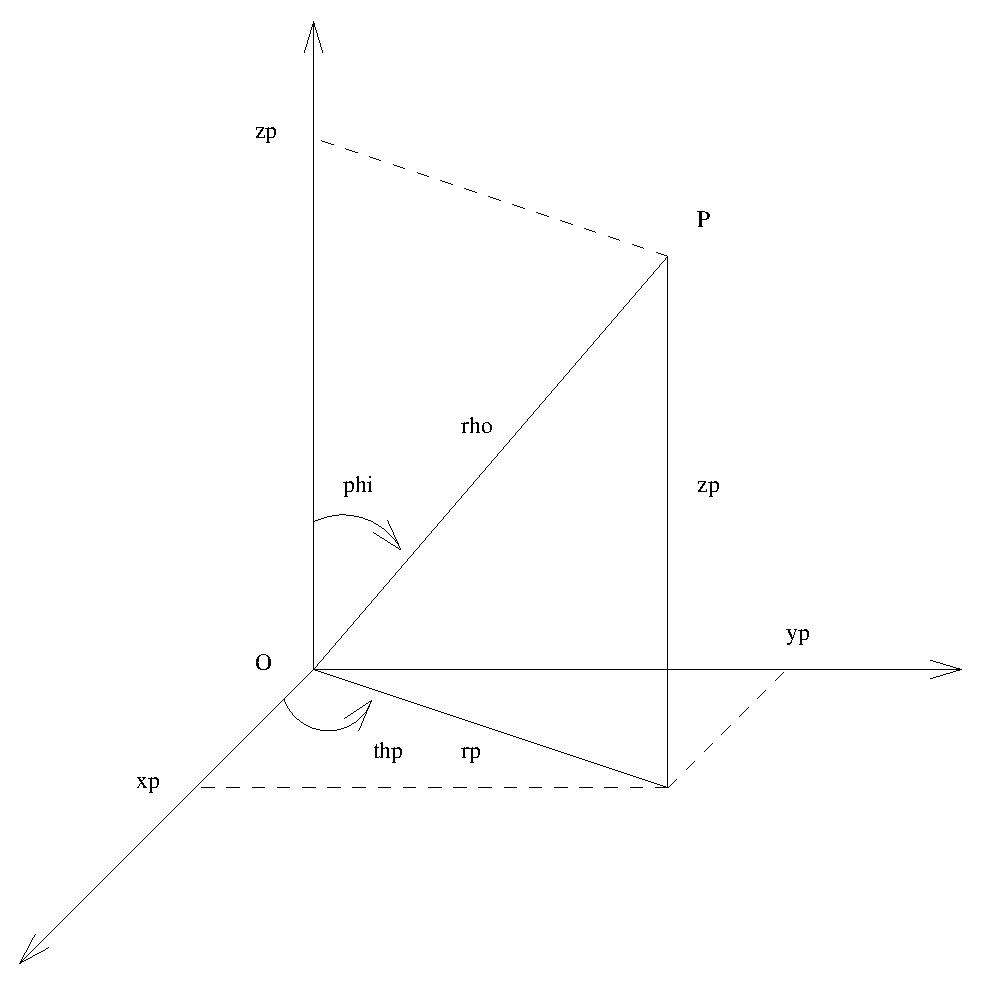
\includegraphics[height=2in]{../../modules/coordinate-systems/pictures/ok-cylindrical-spherical.eps}
\column{0.45\textwidth}
	\begin{itemize}
\item In Cartesian coordinates, a point $P$ is given by triple $(x_P, y_P, z_P)$.
\item<2-> We introduce alternative spherical coordinates $(\rho_P, \phi_P,\theta_P)$.
\begin{itemize}
\item \alert<3>{$\rho_P$: distance $|OP|$;}
\item \alert<4>{$\phi_P$: angle $Oz$ to $OP$;}
\item \alert<5>{$\theta_P$: angle $Ox$ to $OP_{xy}$.}
\end{itemize}
\item<6-> Coordinates range:
\begin{itemize}
\item \alert<7,8>{$\rho$:} \uncover<8->{\alert<8>{ $[0,\infty)$;}}
\item \alert<9,10>{$\phi$:}  \uncover<10->{\alert<10>{$[0, \pi]$;}}
\item \alert<11,12>{$\theta$:}  \uncover<12->{ \alert<12>{$[0,2\pi)$.}}
\end{itemize}
\end{itemize}
\end{columns}
\end{frame}
%\begin{frame}
\frametitle{Spherical curvilinear ``boxes''}


\begin{columns}
\column{0.4\textwidth}

\psset{xunit=1.5cm, yunit=1.5cm}
\begin{pspicture}(-2, -2)(2,2)
\tiny
\renewcommand{\fcScreen}{[-5 1 -2.4] 0}
\pstVerb{10 dict begin%
/rhoMin 1 def%
/rhoMax 2 def%
/thetaMin 20 def%
/thetaMax 70 def%
/phiMin 20 def%
/phiMax 70 def%
/xSph {theta cos phi sin rho mul mul} def%
/ySph {theta sin phi sin rho mul mul} def%
/zSph {phi cos rho mul} def%
}%
\fcAxesIIId{2}{2}{2}
\uncover<10->{
\pscustom*[linecolor=pink]{%
\fcCurveIIId{phiMin}{phiMax}{ 3 dict begin /rho rhoMin def /phi t def /theta thetaMin def xSph ySph zSph end}
\fcCurveIIId{rhoMin}{rhoMax}{ 3 dict begin /rho t def /phi phiMax def /theta thetaMin def xSph ySph zSph end}
\fcCurveIIId{thetaMin}{thetaMax}{ 3 dict begin /rho rhoMax def /phi phiMax def /theta t def xSph ySph zSph end}
\fcCurveIIId{phiMax}{phiMin}{ 3 dict begin /rho rhoMax def /phi t def /theta thetaMax def xSph ySph zSph end}
\fcCurveIIId{thetaMax}{thetaMin}{ 3 dict begin /rho rhoMax def /phi phiMin def /theta t def xSph ySph zSph end}
\fcCurveIIId{rhoMax}{rhoMin}{ 3 dict begin /rho t def /phi phiMin def /theta thetaMin def xSph ySph zSph end}
}%
}%
\fcLineIIId[linestyle=dashed]{[0 0 0]}{[0 2 0]}

\uncover<7->{\fcCurveIIId{rhoMin}{rhoMax}{ 3 dict begin /rho t def /phi phiMin def /theta thetaMin def xSph ySph zSph end}}
\uncover<5->{\fcCurveIIId{rhoMin}{rhoMax}{ 3 dict begin /rho t def /phi phiMax def /theta thetaMin def xSph ySph zSph end}}
\uncover<9->{\fcCurveIIId[linestyle=dashed, linecolor=red]{rhoMin}{rhoMax}{ 3 dict begin /rho t def /phi phiMin def /theta thetaMax def xSph ySph zSph end}}
\uncover<9->{\fcCurveIIId[linestyle=dashed, linecolor=red]{rhoMin}{rhoMax}{ 3 dict begin /rho t def /phi phiMax def /theta thetaMax def xSph ySph zSph end}}

\uncover<8->{%
\fcCurveIIId[linestyle=dashed, dash = 2.6pt,  linecolor=red] {thetaMin}{thetaMax}{ 3 dict begin /rho rhoMin def /phi phiMin def /theta t def xSph ySph zSph end}
\fcCurveIIId{thetaMin}{thetaMax}{ 3 dict begin /rho rhoMax def /phi phiMin def /theta t def xSph ySph zSph end}
\fcCurveIIId[linestyle=dashed, linecolor=red]{thetaMin}{thetaMax}{ 3 dict begin /rho rhoMin def /phi phiMax def /theta t def xSph ySph zSph end}
\fcCurveIIId{thetaMin}{thetaMax}{ 3 dict begin /rho rhoMax def /phi phiMax def /theta t def xSph ySph zSph end}
}%

\uncover<4->{\fcCurveIIId{phiMin}{phiMax}{ 3 dict begin /rho rhoMin def /phi t def /theta thetaMin def xSph ySph zSph end}}
\uncover<9->{\fcCurveIIId[linestyle=dashed, linecolor=red]{phiMin}{phiMax}{ 3 dict begin /rho rhoMin def /phi t def /theta thetaMax def xSph ySph zSph end}}
\uncover<6->{\fcCurveIIId{phiMin}{phiMax}{ 3 dict begin /rho rhoMax def /phi t def /theta thetaMin def xSph ySph zSph end}}
\uncover<9->{\fcCurveIIId{phiMin}{phiMax}{ 3 dict begin /rho rhoMax def /phi t def /theta thetaMax def xSph ySph zSph end}}
\pstVerb{end}
\end{pspicture}

\psset{xunit=1cm, yunit=1cm}
\begin{pspicture}(-2, -2)(2,2)
\tiny
\pstVerb{10 dict begin%
/rhoMin 1 def%
/rhoMax 2 def%
/thetaMin 20 57.2957795 div def%
/thetaMax 70 57.2957795 div  def%
/phiMin 20 57.2957795 div def%
/phiMax 70 57.2957795 div def%
}%
\fcAxesIIId[arrows=->, xLabel=$~~\rho$, yLabel=$~~\phi$, zLabel=$~~\theta$]{2.5}{3.8}{2.5}
\pscustom*[linecolor=cyan]{%
\fcPolyLineIIId{[rhoMin phiMin thetaMin] [rhoMax phiMin thetaMin] [rhoMax phiMax thetaMin] [rhoMax phiMax thetaMax] [rhoMin phiMax thetaMax] [rhoMin phiMin thetaMax] [rhoMin phiMin thetaMin]}
}
\fcLineIIId[linestyle=dashed]{[0 0 0]}{[0 3.8 0]}
\fcDotIIId{[rhoMin 0 0 ]}
\fcPutIIId[t]{[rhoMin 0 -0.2 ]}{$\rho_{min}$}
\fcDotIIId{[rhoMax 0 0 ]}
\fcPutIIId[t]{[rhoMax 0 -0.2 ]}{$\rho_{max}$}
\fcDotIIId{[0 0 thetaMin  ]}
\fcPutIIId[r]{[0 0 thetaMin]}{$\theta_{min}~~$}
\fcDotIIId{[0 0 thetaMax]}
\fcPutIIId[r]{[0 0 thetaMax]}{$\theta_{max}~~$}
\fcDotIIId{[0  phiMin 0  ]}
\fcPutIIId[b]{[0 phiMin 0.2 ]}{$~\phi_{min}$}
\fcDotIIId{[0  phiMax 0  ]}
\fcPutIIId[b]{[0 phiMax 0.2 ]}{$\phi_{max}$}

\fcLineIIId[linecolor=blue, linestyle=dashed]{[rhoMin phiMax thetaMin]}{[rhoMax phiMax thetaMin]}
\uncover<5-9>{\fcLineIIId[linecolor=red, linewidth=2pt, linestyle=dashed]{[rhoMin phiMax thetaMin]}{[rhoMax phiMax thetaMin]}}
\fcLineIIId[linecolor=blue]{[rhoMax phiMax thetaMin]}{[rhoMax phiMin thetaMin]}
\uncover<6-9>{\fcLineIIId[linecolor=red, linewidth=2pt]{[rhoMax phiMax thetaMin]}{[rhoMax phiMin thetaMin]}
}
\fcLineIIId[linecolor=blue]{[rhoMax phiMin thetaMin]}{[rhoMin phiMin thetaMin]}
\uncover<7-9>{\fcLineIIId[linecolor=red, linewidth=2pt]{[rhoMax phiMin thetaMin]}{[rhoMin phiMin thetaMin]}}
\fcLineIIId[linecolor=blue, linestyle=dashed]{[rhoMin phiMin thetaMin]}{[rhoMin phiMax thetaMin]}
\uncover<4-9>{\fcLineIIId[linecolor=red, linewidth=2pt, linestyle=dashed]{[rhoMin phiMin thetaMin]}{[rhoMin phiMax thetaMin]}}

\fcLineIIId[linecolor=blue, linestyle=dashed]{[rhoMin phiMax thetaMax]}{[rhoMin phiMax thetaMin]}
\fcLineIIId[linecolor=blue]{[rhoMax phiMax thetaMax]}{[rhoMax phiMax thetaMin]}
\fcLineIIId[linecolor=blue]{[rhoMax phiMin thetaMax]}{[rhoMax phiMin thetaMin]}
\fcLineIIId[linecolor=blue]{[rhoMin phiMin thetaMax]}{[rhoMin phiMin thetaMin]}
\uncover<8-9>{%
\fcLineIIId[linecolor=red, linestyle=dashed, linewidth=2pt]{[rhoMin phiMax thetaMax]}{[rhoMin phiMax thetaMin]}
\fcLineIIId[linecolor=red, linewidth=2pt]{[rhoMax phiMax thetaMax]}{[rhoMax phiMax thetaMin]}
\fcLineIIId[linecolor=red, linewidth=2pt]{[rhoMax phiMin thetaMax]}{[rhoMax phiMin thetaMin]}
\fcLineIIId[linecolor=red, linewidth=2pt]{[rhoMin phiMin thetaMax]}{[rhoMin phiMin thetaMin]}
}%
\fcLineIIId[linecolor=blue]{[rhoMin phiMax thetaMax]}{[rhoMax phiMax thetaMax]}
\fcLineIIId[linecolor=blue]{[rhoMax phiMax thetaMax]}{[rhoMax phiMin thetaMax]}
\fcLineIIId[linecolor=blue]{[rhoMax phiMin thetaMax]}{[rhoMin phiMin thetaMax]}
\fcLineIIId[linecolor=blue]{[rhoMin phiMin thetaMax]}{[rhoMin phiMax thetaMax]}
\uncover<9>{%
\fcLineIIId[linecolor=red, linewidth=2pt]{[rhoMin phiMax thetaMax]}{[rhoMax phiMax thetaMax]}
\fcLineIIId[linecolor=red, linewidth=2pt]{[rhoMax phiMax thetaMax]}{[rhoMax phiMin thetaMax]}
\fcLineIIId[linecolor=red, linewidth=2pt]{[rhoMax phiMin thetaMax]}{[rhoMin phiMin thetaMax]}
\fcLineIIId[linecolor=red, linewidth=2pt]{[rhoMin phiMin thetaMax]}{[rhoMin phiMax thetaMax]}
}%
\pstVerb{end}
\end{pspicture}

\column{0.6\textwidth}
\begin{itemize}
\item Cut off a rectangular box $B$ in the $\rho, \phi, \theta$-coordinates. 
$
B:=\left\{(\rho, \phi, \theta) |\left| \begin{array}{ccccc} 
\rho_{min} &\leq& \rho &\leq& \rho_{max} \\
\phi_{min} &\leq& \phi &\leq& \phi_{max}\\
\theta_{min} &\leq& \theta &\leq& \theta_{max}\\
\end{array}\right.\right\}
$
\item<2-> As $(\rho, \phi, \theta)$ traverse $B$, the point $P(\rho, \phi,\theta)$ traverses curvilinear ``box'' $Y$: %in the $x,y,z$-coordinates: 
\[
Y = \left\{ P(\rho, \phi, \theta) | (\rho, \phi, \theta)\in B \right\}.
\]
\item<3-> \alert<3-10>{ What is the shape of that curvilinear box?}
\item<11-> What is the volume?
\end{itemize}
\end{columns}
\end{frame}

}
\end{document}
